\documentclass[nobib]{tufte-handout}

%\\geometry{showframe}% for debugging purposes -- displays the margins

\newcommand{\bra}[1]{\left(#1\right)}
\usepackage{amssymb}
\usepackage{hyperref}
\usepackage{pgfplots}
\usepackage[activate={true,nocompatibility},final,tracking=true,kerning=true,spacing=true,factor=1100,stretch=10,shrink=10]{microtype}
\usepackage{color}
\usepackage{steinmetz}
% Fixes captions and images being cut off
\usepackage{marginfix}
\usepackage{array}
\usepackage{tikz}
\usepackage{amsmath,amsthm}
\usetikzlibrary{shapes}
\usetikzlibrary{positioning}
\usepackage{listings}
\usepackage{caption}
\DeclareCaptionFont{white}{\color{white}}
\DeclareCaptionFormat{listing}{\colorbox{gray}{\parbox{\textwidth}{#1#2#3}}}
\captionsetup[lstlisting]{format=listing,labelfont=white,textfont=white}

% Set up the images/graphics package
\usepackage{graphicx}
\setkeys{Gin}{width=\linewidth,totalheight=\textheight,keepaspectratio}
\graphicspath{{.}}

\title{Notes for MA 26500 - Linear Algebra I}
\author[Shubham Saluja Kumar Agarwal]{Shubham Saluja Kumar Agarwal}
\date{\today}  % if the \date{} command is left out, the current date will be used

% The following package makes prettier tables.  We're all about the bling!
\usepackage{booktabs}

% The units package provides nice, non-stacked fractions and better spacing
% for units.
\usepackage{units}

% The fancyvrb package lets us customize the formatting of verbatim
% environments.  We use a slightly smaller font.
\usepackage{fancyvrb}
\fvset{fontsize=\normalsize}

% Small sections of multiple columns
\usepackage{multicol}

% For finite state machines 
\usetikzlibrary{automata} % Import library for drawing automata
\usetikzlibrary{positioning} % ...positioning nodes
\usetikzlibrary{arrows} % ...customizing arrows
\tikzset{node distance=2.5cm, % Minimum distance between two nodes. Change if necessary.
    every state/.style={ % Sets the properties for each state
    semithick,
    fill=gray!10},
    initial text={}, % No label on start arrow
    double distance=2pt, % Adjust appearance of accept states
    every edge/.style={ % Sets the properties for each transition
    draw,
    ->,>=stealth', % Makes edges directed with bold arrowheads
    auto,
    semithick}}
\let\epsilon\varepsilon

% These commands are used to pretty-print LaTeX commands
\newcommand{\doccmd}[1]{\texttt{\textbackslash#1}}% command name -- adds backslash automatically
\newcommand{\docopt}[1]{\ensuremath{\langle}\textrm{\textit{#1}}\ensuremath{\rangle}}% optional command argument
\newcommand{\docarg}[1]{\textrm{\textit{#1}}}% (required) command argument
\newenvironment{docspec}{\begin{quote}\noindent}{\end{quote}}% command specification environment
\newcommand{\docenv}[1]{\textsf{#1}}% environment name
\newcommand{\docpkg}[1]{\texttt{#1}}% package name
\newcommand{\doccls}[1]{\texttt{#1}}% document class name
\newcommand{\docclsopt}[1]{\texttt{#1}}% document class option name

% Define a custom command for definitions and biconditional
\newcommand{\defn}[2]{\noindent\textbf{#1}:\ #2}
\let\biconditional\leftrightarrow

\begin{document}

\maketitle

\begin{abstract}
    These are lecture notes for spring 2024 MA 26500 at Purdue. Modify, use, and distribute as you please.
\end{abstract}

\tableofcontents

\section{Course Introduction}
This course serves as an introduction to the fundamental concepts and
applications of linear algebra, a branch of mathematics that explores vector
spaces, linear transformations, and systems of linear equations.

\pagebreak

\section{Systems of Equations in Linear Algebra}
A linear equation is an equation of the form:
\begin{equation*}
    a_1x_1+a_2x_2+...+a_nx_n=b
\end{equation*}
Where $a_1$, $a_2$... and $b$ are given constants.
Note that the exponents of all x terms is 1.
Some examples are:
\begin{equation*}
    2x_1+3x_2=4
\end{equation*}
\begin{equation*}
    5x_1+6x_2=10
\end{equation*}
as opposed to
\begin{equation*}
    2x_1x_2+x_3=9
\end{equation*}
\begin{equation*}
    2x_1+\sqrt{x_2}=8
\end{equation*}
A system of equations is a collection of one or more linear equations involving the same variable set.
An example of this would be:
$$ \begin{cases}
        3x_1 + 5x_2 + x_3 = 3  \\
        7x_1 - 2x_2 + 4x_3 = 4 \\
        -6x_1 + 2x_3 = 2
    \end{cases} $$
where the constant coefficient of $x_2$ in the third equation is 0.\\
A solution is a list of numbers $(s_1, s_2, ..., s_n)$ that makes each equation a true statement when we replace $x_1=s_1$, $x_2=s_2$, ... $x_n=s_n$.
If we have a system of two linear equations, the solution will be the intersection of the two lines that define the equations on the cartesian plane. The system of equations
\begin{align*}
    3x_1-x_2   & = 5 \\
    16x_1-2x_2 & = 6
\end{align*}
is mapped to the following graph:
\begin{center}
    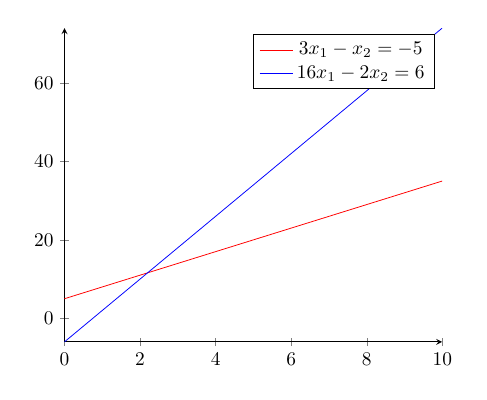
\begin{tikzpicture}[scale = 0.7]
        \begin{axis}[
                axis lines = left,
            ]
            \addplot [
                domain=0:10,
                samples=100,
                color=red,
            ]
            {3*x + 5};
            \addlegendentry{\(3x_1-x_2=-5\)}
            \addplot [
                domain=0:10,
                samples=100,
                color=blue,
            ]
            {8*x - 6};
            \addlegendentry{\(16x_1-2x_2=6\)}

        \end{axis}
    \end{tikzpicture}
\end{center}

There are three kinds of systems:
\begin{enumerate}
    \item One solution
    \item Infinitely many solutions
    \item No solutions
\end{enumerate}
The above example has one solution. This is the intersection of the two lines. This could be further generalized to have far more dimensions as well as far more variables, but such systems are no longer representable in the number of dimensions we can perceive.\\
However, if the lines were parallel, the other two possibilities surge. If the equations are linearly dependent, there would be infinitely many solutions. However, if the value of $b$ were different for the two, while all the variable coefficients were linearly dependent, it would have none.\\
The following is an example of no solution:
\begin{center}
    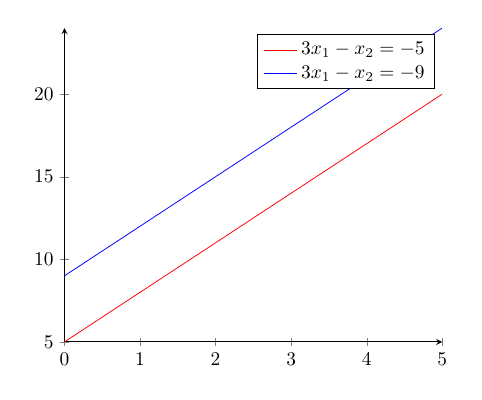
\begin{tikzpicture}[scale = 0.7]
        \begin{axis}[
                axis lines = left,
            ]
            \addplot [
                domain=0:5,
                samples=100,
                color=red,
            ]
            {3*x + 5};
            \addlegendentry{\(3x_1-x_2=-5\)}
            \addplot [
                domain=0:5,
                samples=100,
                color=blue,
            ]
            {3*x + 9};
            \addlegendentry{\(3x_1-x_2=-9\)}
        \end{axis}
    \end{tikzpicture}
\end{center}
While this is infinitely many solutions:
\begin{center}
    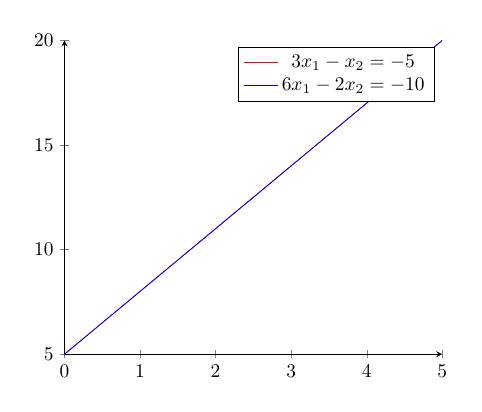
\begin{tikzpicture}[scale = 0.7]
        \begin{axis}[
                axis lines = left,
            ]
            \addplot [
                domain=0:5,
                samples=100,
                color=red,
            ]
            {3*x + 5};
            \addlegendentry{\(3x_1-x_2=-5\)}
            \addplot [
                domain=0:5,
                samples=100,
                color=blue,
            ]
            {3*x + 5};
            \addlegendentry{\(6x_1-2x_2=-10\)}
        \end{axis}
    \end{tikzpicture}
\end{center}
Any system of equations has a matrix notation. For example, the above system can be represented as the following.\\
\begin{equation*}
    \begin{bmatrix}
        3  & -1 & -5 \\
        16 & -2 & 6
    \end{bmatrix}
\end{equation*}
Which has the coefficients of the x values as the first n values, and the value of b as the last one. This is called the augmented matrix of the system of equations. As opposed to:
\begin{equation*}
    \begin{bmatrix}
        3  & -1 \\
        16 & -2
    \end{bmatrix}
\end{equation*}
which is the coefficient matrix.\\
These systems can be solved using the three elementary row operations. This is called row reduction.\\
The three rules are:
\begin{enumerate}
    \item Interchange: Exchange the positions of any two rows
    \item Multiply: Multiply any row by a constant
    \item Addition: Replace the value of a row, with its sum and that of one of the other
          rows multiplied by a scalar.
\end{enumerate}
By using these three rules, one can reduce it to the following form:
\begin{equation*}
    \begin{bmatrix}
        1 & a_2 & a_3 & a_4 \\
        0 & 1   & b_3 & b_4 \\
        0 & 0   & 1   & c_4
    \end{bmatrix}
\end{equation*}
This will result in a trivially solvable unique-solution system of equations. This is also known as a \textbf{consistent} system of equations. We can substitute the value of $x_3$, which is $c_4$, into the equation in the row above, and solve it, as it willnow be a single equation with a single variable. This can be done sequentially until all values are found.\\~\\
Note: If the resulting form is instead
\begin{equation*}
    \begin{bmatrix}
        1 & a_2 & a_3 & a_4 \\
        0 & 1   & b_3 & b_4 \\
        0 & 0   & 0   & c_4
    \end{bmatrix}
\end{equation*}
with $c_4 \neq 0$, there would be no solutions, also known as an \textbf{inconsistent} system. On the other hand, if $c_4 = 0$, there will be infinitely many solutions, but it will still be considered a \textbf{consistent} system.
Another point to note is that if the augmented matrices of two systems of equations are equivalent,
that is, if you can transform one matrix into the other through elementary row operations, the systems of equations will have the same solutions.
\pagebreak
\section{Row Reduction and Echelon Forms}
The leading entry of a row refers to the left-most non zero element in a row.
Thus, the leading entries in the following matrix are:
\begin{equation*}
    \begin{bmatrix}
        \textbf{1} & 2          & 3          & 4 \\
        0          & \textbf{6} & 9          & 6 \\
        0          & 0          & \textbf{8} & 7
    \end{bmatrix}
\end{equation*}
A matrix is in reduced echelon form (REF) if it has the following three properties:
\begin{enumerate}
    \item All non-zero rows are above any rows of all zeros.
    \item Each leading entry in a row is in a column to the right of the leading entry in
          the column above it.
    \item All entries below a leading entry are zeros.\\~\\ If it has the following two
          properties, it will be a row reduced echelon form (RREF):
    \item The leading entry in each non-zero row is 1.
    \item Each leading 1 is the only non-zero element in its column.
\end{enumerate}
Example of echelon form:
\begin{equation*}
    \begin{bmatrix}
        1 & 2 & 5 & 8 \\
        0 & 3 & 9 & 6 \\
        0 & 0 & 9 & 7 \\
        0 & 0 & 0 & 0
    \end{bmatrix}
\end{equation*}
Example of REF:
\begin{equation*}
    \begin{bmatrix}
        1 & 0 & 0 & 8 \\
        0 & 1 & 0 & 6 \\
        0 & 0 & 1 & 7 \\
        0 & 0 & 0 & 0
    \end{bmatrix}
\end{equation*}
\vspace{0.2cm}\\
\textbf{Theorem:} Each matrix is equivalent to one and only one RREF.\\
\quad A pivot position is a location in a matrix that corresponds to a leading 1 in the RREF of a matrix.\\
\quad A pivot column is a column that contains a pivot position.\\~\\
\textit{Tip:} if there is a 1 in the first positions of a row, when the matrix is first "observed", it should be moved to the top of the matrix, as it will most probably make all subsequent computations much easier. \\~\\
\begin{minipage}{\textwidth}
    Row reduction algorithm:
    \begin{enumerate}
        \item Begin with the leftmost non-zero position, and make it the first pivot
              position.
        \item Make all positions under the selected pivot position 0.
        \item Interchange columns to make sure that the rows with the most leading zeros are
              closest to the bottom
        \item Cover the first column and row, and repeat steps 1 to 3 on the resulting
              matrix.
        \item Beginning with the rightmost pivot and working upward and to the left, create
              zeros above each pivot.
    \end{enumerate}
\end{minipage}
\vspace{0.2cm}\\
The solution of the RREF is the solution of the system of equations that has an augmented matrix with the aforementioned RREF.\\
\quad Another thing we can note is that all pivot positions refer to basic variables. If there are any non-pivot columns, the variable referring to these columns will be free, as it will imply that all elements within the column are 0.
\end{document}